%
% latex-sample.tex
%
% This LaTeX source file provides a template for a typical research paper.
%

%
% Use the standard article template.
%
\documentclass{article}

% The geometry package allows for easy page formatting.
\usepackage{geometry}
\geometry{letterpaper}

% Load up special logo commands.
\usepackage{doc}
\usepackage{cite}
\usepackage[margin=1cm]{caption}

% Package for formatting URLs.
\usepackage{url}

% Packages and definitions for graphics files.
\usepackage{graphicx}
\usepackage{epstopdf}
\DeclareGraphicsRule{.tif}{png}{.png}{`convert #1 `dirname #1`/`basename #1 .tif`.png}

%
% Set the title, author, and date.
%
\title{Usability of Modern Display Technologies}
\author{Rachel Rivera}
\date{October 16, 2014}

%
% The document proper.
%
\begin{document}

% Add the title section.
\maketitle

% Add an abstract.
\abstract{
This study aims to examine how interaction design concepts specifically map to the usability of modern display technology.
//TODO: write a better abstract
}

% Add various lists on new pages.
\pagebreak
\tableofcontents


% Start the paper on a new page.
\pagebreak

%
% Body text.
%
\section{Introduction}
\label{introduction}

Electronic screens are the devices through which information is transferred between the user and the interface. Although electronic displays have been around for roughly a century,\footnote{One of the earliest electronic displays, the cathode ray tube (CRT),  was first made commercial in 1922.\cite{Cathode}} they are still transforming and evolving in a multitude of ways. Screens are diversifying in order to tackle the limitations that have presented themselves over the years.\cite{Eisenberg} Screen devices have been changing in size, shape, flexibility, and resolution in order to improve usability for specific tasks. For example, \textit{focus plus context screens}, which are wall-size low-resolution displays with an embedded high-resolution display region, are currently a proposed solution to working with visual documents too large to fit standard screens.\cite{Baudisch} Another kind of screen that is emerging is the \textit{BiDirectional (BiDi) Screen}, which is a thin, depth-sensing liquid-crystal display (LCD) that allows for 3D interaction using light fields.\cite{Hirsch} 

 Though each kind of screen has its merits, this study will focus exclusively on touch sensitive screens. In a study from Link\"{o}ping University, researchers articulated how ``interaction on touch sensitive screens is literally the most `direct' form of HCI, where information display and control are but one surface."\cite{Albinsson} Though it is clear that a connection between modern touchscreen devices and the field of interaction design exists, this study aims to investigate exactly \textit{how} interaction design concepts specifically map to the usability of touch screens. 


\section{Background/ Prior Work/ Literary Review}
\subsection{Limitations/Proposed Solutions}
There exists a fair amount of previous work pertaining to the usability of touch sensitive screens. The literature often evaluates usability by examining the limitations of these screen devices. One limitation that is discussed in the literature is how typing on flat surfaces---with no physical keys to guide the fingers---requires heightened visual attention. A study by Hussain Tinwala and Scott MacKenzie suggests that since the visual demand on the user is increased, concentration is diverted from the thoughts being expressed. \cite{Tinwala:2010:ETE:1868914.1868972} The lack of tactile features not only diverts attention from thoughts being expressed, but moreover, it makes the devices difficult to use for Individuals with Blindness or Severe Visual Impairment (IBSVI). A study from Virginia Polytechnic Institute and State University examined how, even with the use of features such as  \textit{VoiceOver}\footnote{\textit{VoiceOver} for OS X tells users what is on the screen and walks users through actions.\cite{VoiceOver}}, touch screens still do not provide sufficient support for IBSVI. These users were only able to ``develop a spatial mental model for the interface or the screen through dead reckoning" since there is an ``absence of any landmark other than the boundary of the device." \cite{El-Glaly:2013:TTF:2460625.2460665} 

One purposed solution to this limitation is a physical overlay, developed by researchers specifically to help IBSVI engage their spatial cognition, perception, and sensing resources while interacting with touch screens.  \cite{El-Glaly:2013:TTF:2460625.2460665} The tactile overlay covers the touch device screen. An IBSVI can use the tactile patterns of the overlay to locate the text, icons, or buttons in the touch device interface. A study examining the efficacy of this physical overlay illustrated that IBSVI who used it were generally more efficient than those using voice-over technology or `trail-and-error' exploration. \cite{El-Glaly:2013:TTF:2460625.2460665}


Another limitation of touchscreen devices that is examined in the literature is how the human finger as a pointing device has ``very low resolution."\cite{Albinsson} With mobile touch screens in particular, research has illustrated the difficulty in pointing at targets that are often smaller than the width of the user's finger. A notable technique was created by Schneiderman, Sears, and colleagues to specifically address this problem.\cite{Sears} Their basic technique provides a cursor above the user's finger tip with a fixed offset when touching the screen. The user drags the cursor to a desired target and then lifts the finger to select the targeted object. Although this technique generally allowed a user to perform precise movements with less errors, the user's efficiency tended to suffer.\cite{Sears}

Many studies have purposed using a stylus (pen) to interact with touch screens instead of using a bare finger. A stylus has better ``resolution" than a finger tip and recent studies have demonstrated that pen input is emerging as a promising interaction modality for touch screens.\cite{Bi} A study by Forlines and Balakrishnan, which evaluated multiple forms of stylus input, articulated that one drawback of this approach is the occlusion of other elements on the screen by the pen.\cite{Forlines}

Zooming is also found in the literature as a proposed solution to increase precision of touchscreen interaction. It is possible to use zooming to enlarge the information space of the touchscreen enough so that the user can comfortably point at the target with a bare finger. However, a study by P\"{a}r-Anders Albinsson and Shumin Zhai asserted that zooming has a fundamental drawback since ``when zoomed to a sub area of interest, one loses the contextual global view that can be important for the user's task."\cite{Albinsson} 

\subsection{Advantages}
Previous work on the subject of touchscreen display devices not only discusses limitations and proposed solutions, but also examines advantages of touchscreen displays. Ben Schneiderman's essay, \textit{Touch Screens Now Offer Compelling Uses}, provides a number of reasons why touchscreen devices can be advantageous: they are forms of direct manipulation, they are easy to learn, they are the fastest pointing device, no extra workspace is required to use them, etc. \cite{73754} Many experiments have been conducted that provide evidence supporting Schneiderman's reasons. For example, the results from an experiment by Robert Hardy and Enrico Rukzio suggest that finger interaction is, in fact, faster than alternative pointing devices in most situations.\cite{Hardy:2008:TIT:1409240.1409267} Schneiderman's assertion that touchscreen display devices are generally more learnable was also supported by an experiment that examined the learnability of a touchscreen electronic medical record system.\cite{Douglas:2011:SUL:2029976.2029990}


\section{Methods}
The prior work in the field demonstrates that there is a variety of different advantages as well as limitations that can be examined when evaluating the usability of touchscreen devices. Since this paper is too short to discuss each advantage and limitation, the paper will focus exclusively on the limitation of the minimal tactile feedback provided by touchscreen devices. 

\subsection{Prevailing Set of Views}
Most research pertaining to this limitation focuses on how the lack of tactile feedback affects the usability of the device for Individuals with Blindness or Severe Visual Impairment. Touch screen interfaces have been popular for over 20 years, and concerns about touch screen accessibility for IBSVI have remained active throughout this time. \cite{Buxton:1986:HID:22339.22386} The prevailing set of views on the subject recognize that the touch screens are not effective for the IBSVI, and propose solutions specifically to address needs of the IBSVI. 

Previous research has explored techniques that make touch screens more accessible by modifying the hardware. This paper mentioned one such technique when explaining physical overlays.\cite{El-Glaly:2013:TTF:2460625.2460665} However, a recent study articulated how hardware modifications ``may be expensive to install, may limit the flexibility of the underlying software (by imposing physical structures), and may interfere with use by sighted people." \cite{Kane:2011:AOI:2047196.2047232}  The study asserts that for these reasons, techniques that rely upon hardware modifications have not been widely adopted.

More recent efforts have focused on using gestures to provide IBSVI with access to touch screens without modifying the underlying hardware. For example, Slide Rule \cite{Kane:2008:SRM:1414471.1414487} used multi-touch gestures to allow blind users to browse and explore content on a touch screen-based smartphone. 

\begin{figure}[ht]
\centering
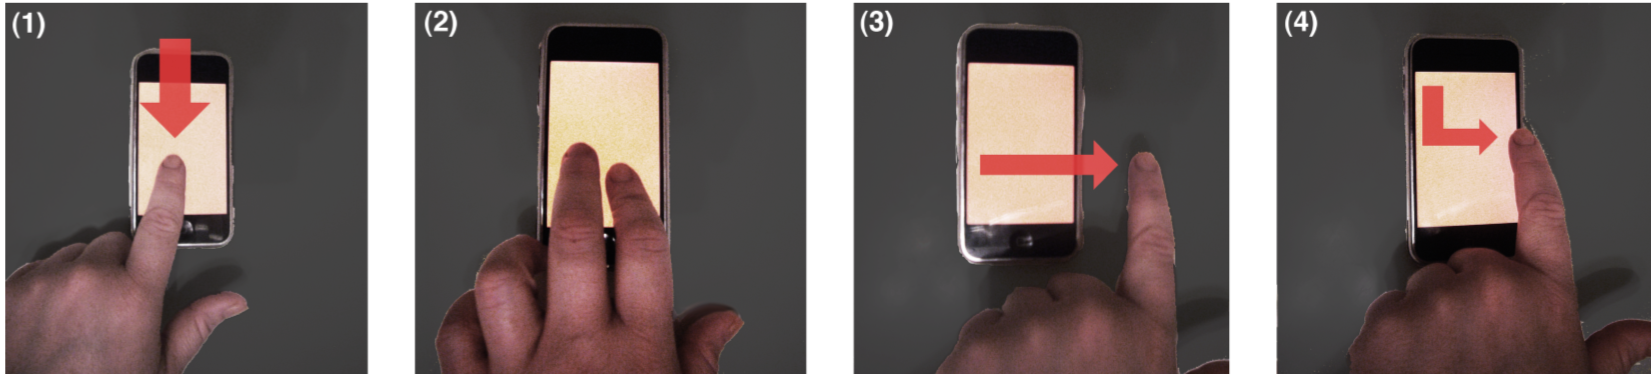
\includegraphics[width=4.5in]{slide-rule.jpg} 
\caption{An example of some multi-touch gestures recognized by Slide Rule.(1) A one-finger scan to browse lists; (2) A two-finger tap to select items; (3) A flick gesture used to flip between pages; (4) An L-select gesture to browse hierarchy of menu options. \cite{Kane:2008:SRM:1414471.1414487} }
\label{figure-sample}
\end{figure}

There exist several input entry methods, however, that attempt to address this problem. For instance, Tinwala and MacKenzie present a system that includes auditory and tactile feedback to guide eyes-free entry using speech and non-speech sounds. \cite{Tinwala:2010:ETE:1868914.1868972} 

  Researchers have also explored techniques to 
address specific aspects of blind touch screen interaction, 
such as text entry and gesture selection\cite{conf/chi/KaneWL11}. 
However, these techniques have often focused on small, 
mobile phone-sized screens. Furthermore, many of these 
techniques change the fundamental layout of the screen to 
improve accessibility. Thus, our current work addresses 
interaction with larger touch screens, and explores methods 
to preserve users’ understanding of the screen layout. 

\clearpage
\subsection{Emerging technology}
There is technology emerging that is not necessarily aimed to specifically help the IBSVI.

Another proposed solution comes from Tactus Technology, a company in Fremont, California. Employees from Tactus Technology are creating a keyboard with shape-shifting keys that pop up from the screen's surface when needed and recede again when no longer necessary.\cite{Tactus} Craig Ciesla, the co-founder of the company, said that the keyboard will be offered later this year. 

\begin{figure}[ht]
\centering
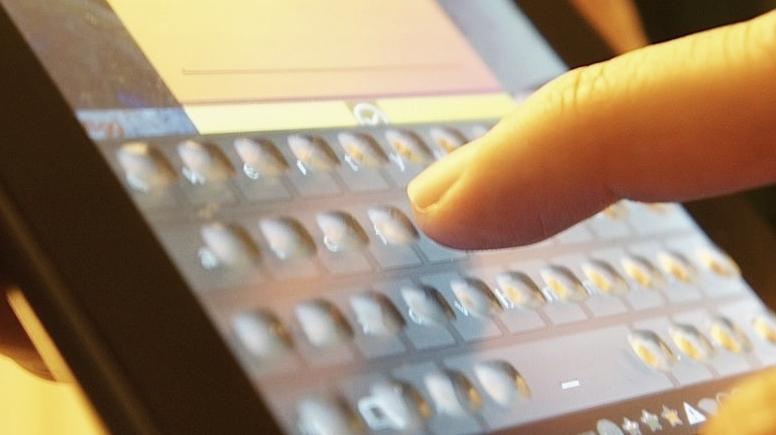
\includegraphics[width=3in]{tactus-keyboard.jpg} 
\caption{A Tactus keyboard}
\label{figure-sample}
\end{figure}
Though literature on the subject of touchscreen display devices have presented many limitations, the most relevant and important seems to be the lack of tactile features and the requirement for heightened visual attention. For people who are blind, accessing touch screen interfaces is nearly impossible. Some accessibility features are beginning to be developed though.

\section{Discussion}
Research discusses usability for IBSVI but does has not delved into technology that can be effective for the sighted and IBSVI alike.
The principle of feedback
feedback ---sending back to the user information about what action has actually been done, what result has been accomplished--- is a well-known concept in the science of control and information theory\cite{Norman02} "In the good old days of the telephone", "telephones were designed with much more care and concern for the user. Designers at the Bell Telephone Laboratories worried a lot about feedback. The push buttons were designed to give an appropriate feel---tactile feedback. When a button was pushed, a tone was fed back into the earpiece so the user could tell that the button had been properly pushed. When the phone call was being connected, clicks, tones, and other noises gave the user feedback about the progress of the call." ``All this changed." ``Why are modern telephone systems so difficult to use? Basically, the problem is that the systems have more features and less feedback"

\section{Conclusions}


Wrap up your paper with an ``executive summary'' of the paper itself, reiterating its subject and its major points.  If you want examples, just look at the conclusions from the literature.
\clearpage


\bibliography{mybib}{}
\bibliographystyle{plain}
\end{document}
%%%%%%%%%%%%% end %%%%%%%%%%%%%%%%%%%%%%%%%%%%%%%


\end{document}
